\chapter{Modeling Component Operations}

In order to describe the modeling and analysis aspects of this tool, consider the following example: 

\section{Trajectory Planning Application}

The component assembly for this application is shown in Figure \ref{fig:tpa}. This application consists of two components: A \emph{Sensor} component and a \emph{Trajectory Planner} component. The Sensor component periodically publishes on a trigger topic, notifying the Trajectory Planner of the existence of new sensor data. Once the notification is received, the Trajectory Planner makes an RMI call to retrieve the data structure of sensor values. Using the updated sensor values, the Trajectory Planner calculates a new trajectory for the satellite. 

\begin{figure}[ht]
\centering
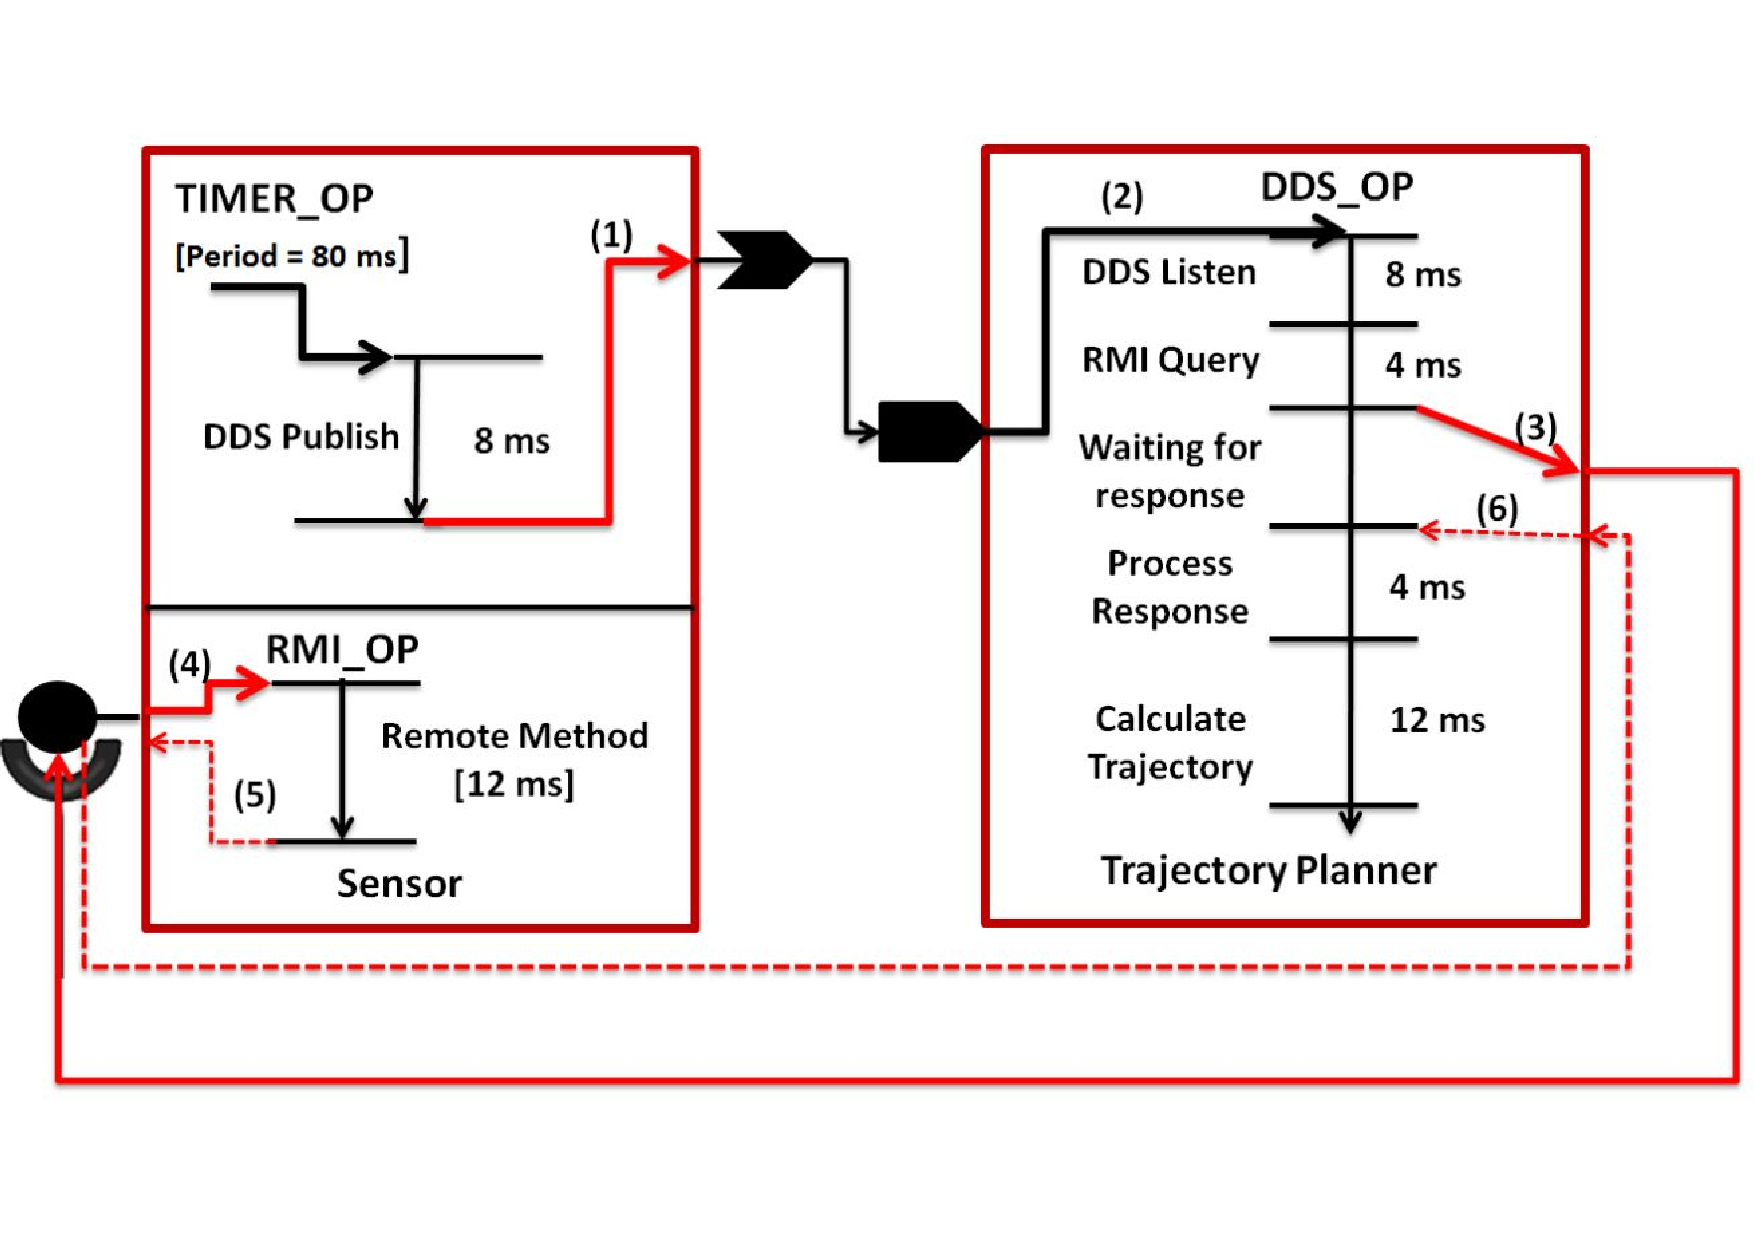
\includegraphics[width=0.88\textwidth]{./figs/CPN_TPA}
\caption{Trajectory Planning Application}
\label{fig:tpa}
\vspace{-0.2in}
\end{figure}
%\vspace{0.1in}

\begin{figure}[ht]
\centering
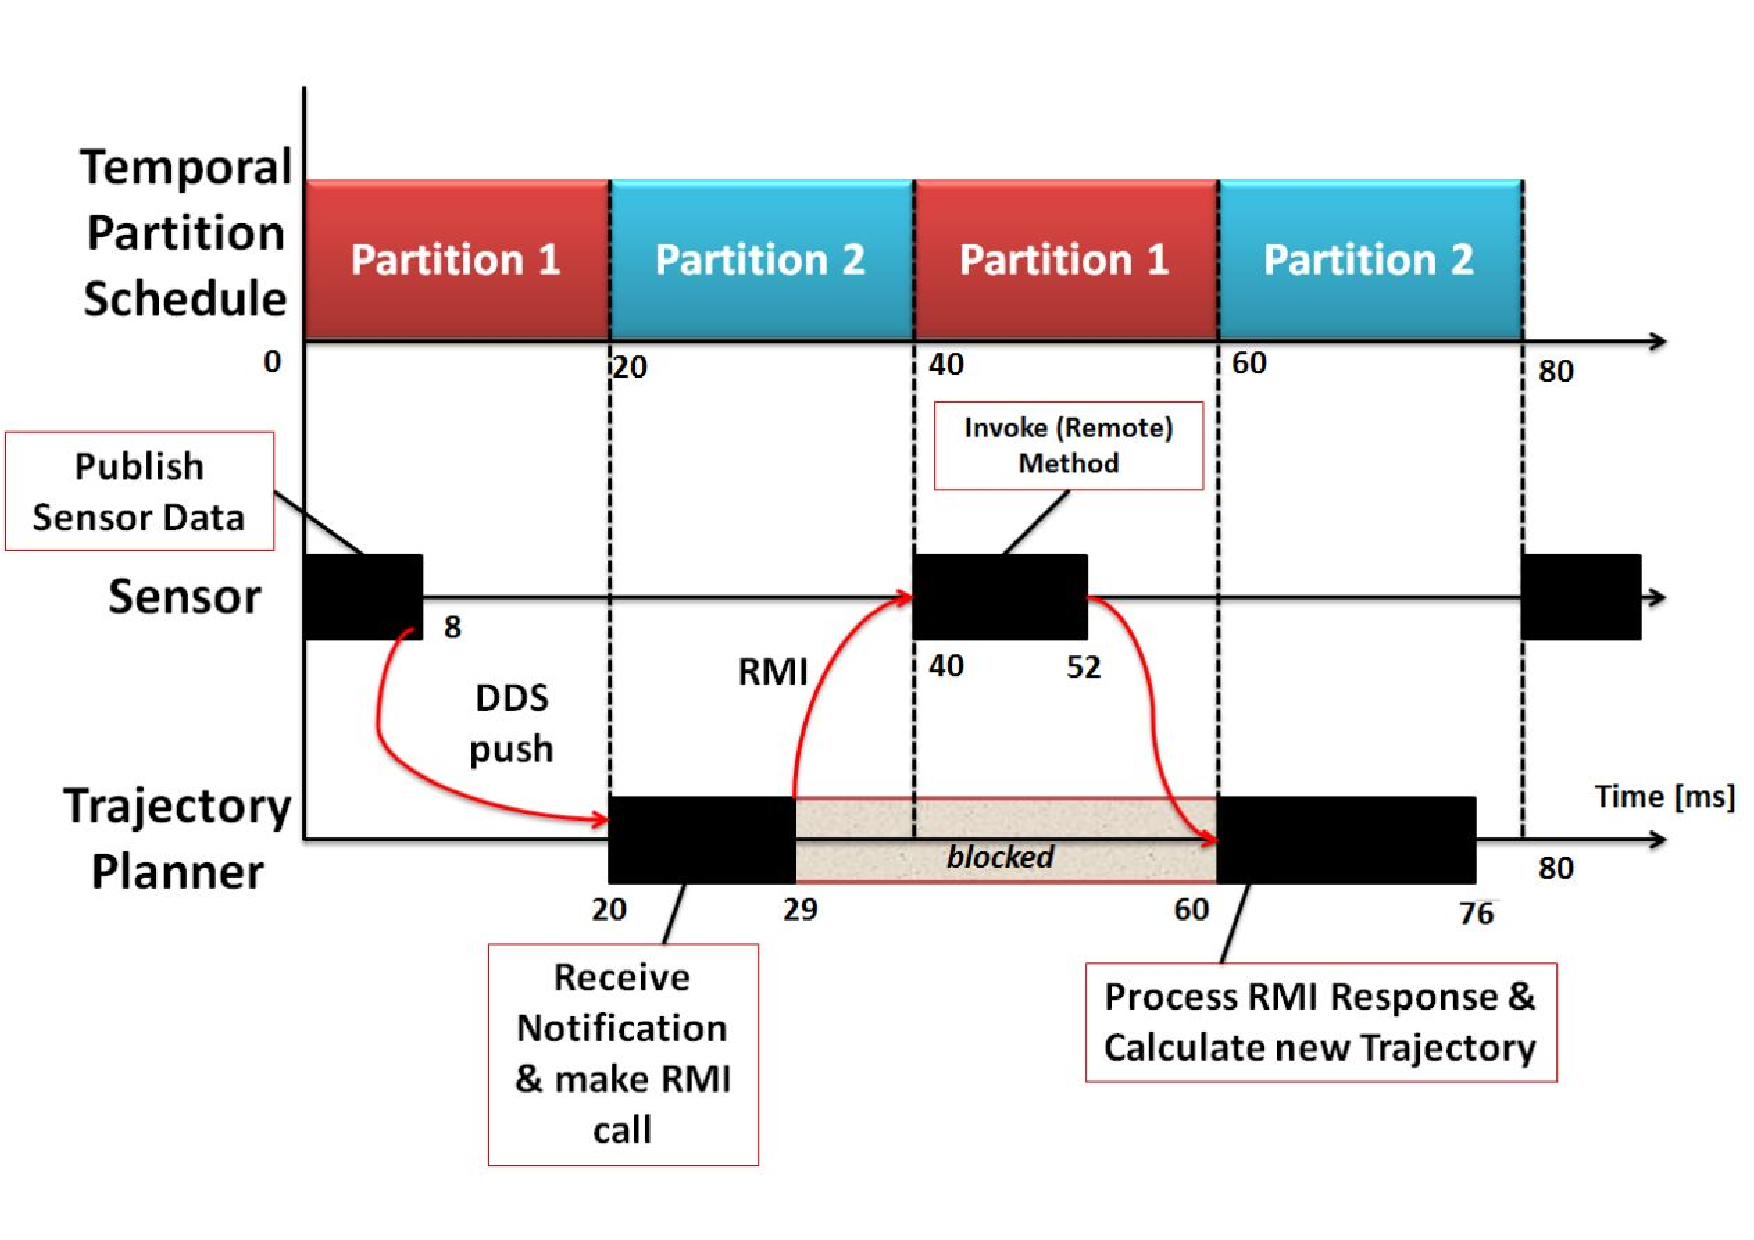
\includegraphics[width=0.8\textwidth]{./figs/CPN_TPA_TD}
\caption{Timing Diagram for Trajectory Planning}
\label{fig:tpa_td}
\vspace{-0.2in}
\end{figure}
\vspace{0.1in}

Figure \ref{fig:tpa_td} shows the partition schedule and temporal behavior considered. The sensor component operates on partition 1, and the trajectory planner operates on partition 2. Both partitions have a duration of 20 ms and a period of 40 ms. The sensor component is associated with a periodic timer that fires every 80 ms. When this timer expires, the sensor component publishes on a notification topic. Accounting for network latencies, the analysis assumes that this task does not take more than 8 ms. Once the notification is sent out, the sensor component becomes passive. With DDS push semantics, this notification manifests itself as a DDS operation on the trajectory planner's message queue. When partition 2 becomes active, the trajectory planner component receives the notification is has subscribed to, after which it makes an RMI call to the sensor component to obtain the updated sensor values. After the RMI call is made, this component blocks for the remainder of the partition. When the sensor component is scheduled again, it services the RMI request and sends out the RMI response, effectively unblocking the trajectory planner. Once the new sensor data is retrieved, the trajectory planner calculates a new trajectory for the satellite node. 

\vspace{0.1in}
\noindent\textbf{Location:}\\
\texttt{\$F6IAP/f6mde/f6ml/IM/samples/CPNAnalysis\_Samples/ \\ Trajectory\_Planning\_Application}
   \texttt{/Scenario\_1\_RMI\_Blocking\_Delay/}
	
\section{Adding BusinessLogic Atoms to Component Ports}

In the F6ML model of the application, \emph{BusinessLogic} atoms can be added to component ports exposed in the Component Implementation. BusinessLogic atoms represent the timing specifications for the operations that are implemented by the component port. For instance - In order to model the timing specification of a timer operation in a component, the first step is to:
\begin{enumerate}
\item Drag a new BusinessLogic atom to the canvas from the Development aspect in the Part Browser inside the Component Implementation.
\item Connect this atom to a \emph{Timer} port exposed on the instance of the Component Definition.
\item The Operations attribute of this BusinessLogic atom represents the timing specification of the timer operation.
\end{enumerate}

Figure \ref{fig:tpa_timerbl} shows a BusinessLogic atom called \emph{Timer\_BL} connected to a timer port \emph{Publish\_Timer} in the Sensor component. Note that the BusinessLogic atom is only visible in the \emph{Development} aspect inside Component Implementation.

\begin{figure}[ht]
\centering
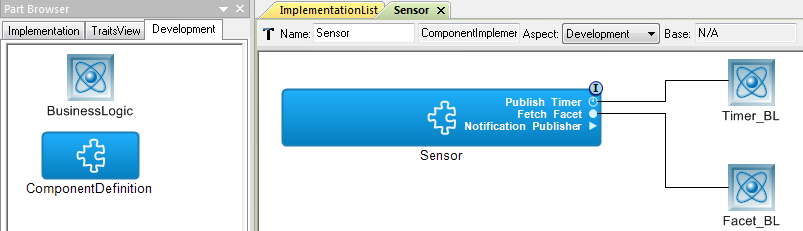
\includegraphics[width=0.99\textwidth]{./figs/TPA_TIMERBL}
\caption{Connecting a BusinessLogic atom to a Component Port}
\label{fig:tpa_timerbl}
\vspace{-0.2in}
\end{figure}
\vspace{0.1in}

\section{ANTLR 4 Grammar for Component Operations}

The timing behavior for business logic of component operations is expressed in the \emph{Operations} attribute of a BusinessLogic atom. This behavior is modeled using a well-defined ANTLR 4 grammar. This section describes the grammar and how it applied is for the trajectory planning application. 

\subsection{Defining the Timing Specification}

The Operations attribute of a BusinessLogic atom consists of one or more \emph{operations}. Each operation: 
\begin{enumerate}
\item Begins with the keyword \emph{'Do'}, followed by
\item The \emph{name} of the component operation, followed by
\item The \emph{priority} of the component operation, followed by
\item The \emph{deadline} of the component operation.
\item One or more operational steps
\end{enumerate}

Note that the priority and deadline of the operation are specified inside square brackets. This is defined in the grammar in Figure \ref{fig:grammar1}.

The name of the component operation is important. For instance - 
\begin{itemize}
\item Every timer operation needs to be called \emph{on\_timer}.
\item Every subscriber operation where the subscriber is configured to be of type \emph{PUSH\_WITHOUT\_INSTANCE\_NOTIFICATIONS} - should be named either \emph{on\_one\_data} or \emph{on\_many\_data}. 
\item Every subscriber operation where the subscriber is configured to be of type \emph{PUSH\_WITH\_INSTANCE\_NOTIFICATIONS} - should be named either \emph{on\_one\_update} or \emph{on\_many\_updates}. 
\item Every facet operation name must match one of the methods defined in the interface that refers the connected facet. 
\end{itemize}

If any of these rules are not followed, the CPNGenerator interpreter will provide a GME Console Error detailing the issue.

\begin{figure}[ht]
\centering
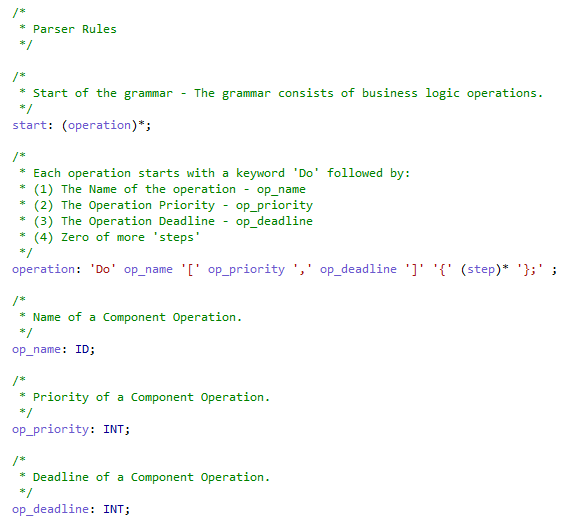
\includegraphics[width=0.99\textwidth]{./figs/Grammar_1}
\caption{Modeling Component Operations}
\label{fig:grammar1}
\vspace{-0.2in}
\end{figure}
\vspace{0.1in}

Note that BusinessLogic atoms can only be connected to the following ports: 
\begin{itemize}
\item Timer ports
\item Push Subscriber ports 
\item Facets
\item AMI Receptacles - describing AMI callback operations
\end{itemize}

As mentioned earlier, every operation is described by the sequence of steps executed in the business logic. As shown in Figure \ref{fig:grammar2}, an operational step can be a (1) Fragment of code, (2) RMI call, (3) AMI call, (4) DDS Publish, (5) DDS Pull Subscribe, (6) DDS Push Subscribe or a (7) Control Loop.

\begin{figure}[ht]
\centering
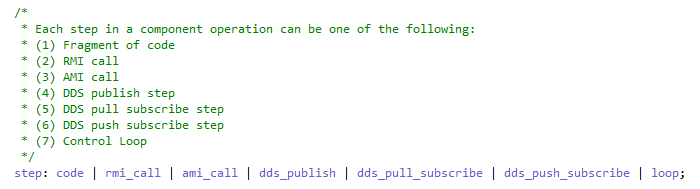
\includegraphics[width=0.99\textwidth]{./figs/Grammar_2}
\caption{Operational steps}
\label{fig:grammar2}
\vspace{-0.2in}
\end{figure}
\vspace{0.1in}

Figures \ref{fig:code_fragment}. \ref{fig:grammar3}, \ref{fig:grammar4}, \ref{fig:grammar5}, \ref{fig:grammar6} and \ref{fig:grammar7} show how the different operational steps are defined in the Business Logic grammar. 

\subsection{Code Fragment}

\begin{figure}[ht]
\centering
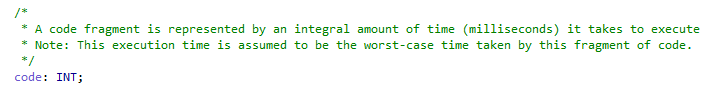
\includegraphics[width=0.99\textwidth]{./figs/Grammar_code}
\caption{Code Fragment}
\label{fig:code_fragment}
\vspace{-0.2in}
\end{figure}
\vspace{0.1in}



\subsection{RMI call}

\begin{figure}[ht]
\centering
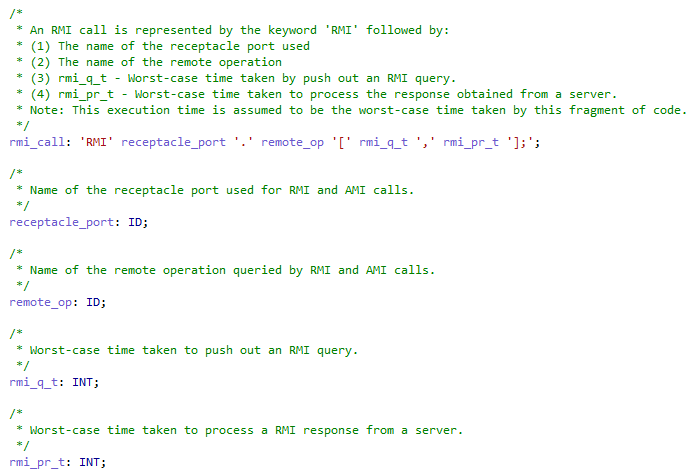
\includegraphics[width=0.99\textwidth]{./figs/Grammar_3}
\caption{RMI call}
\label{fig:grammar3}
\vspace{-0.2in}
\end{figure}
\vspace{0.1in}

\subsection{AMI call}

\begin{figure}[ht]
\centering
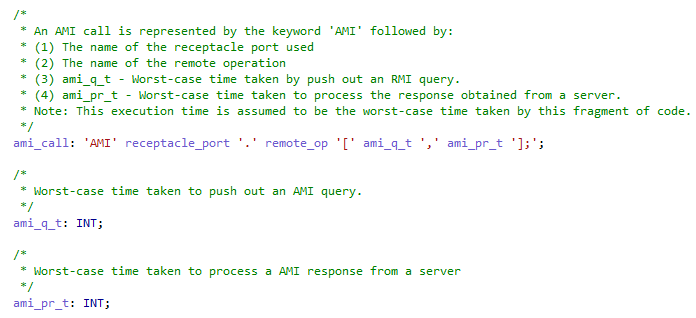
\includegraphics[width=0.99\textwidth]{./figs/Grammar_4}
\caption{AMI call}
\label{fig:grammar4}
\vspace{-0.2in}
\end{figure}
\vspace{0.1in}

\subsection{DDS Publish}

\begin{figure}[ht]
\centering
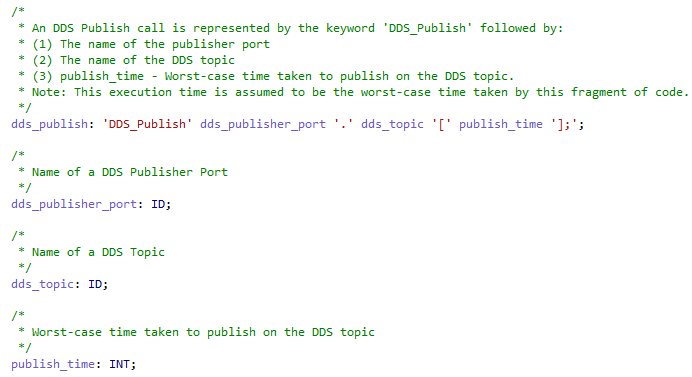
\includegraphics[width=0.99\textwidth]{./figs/Grammar_5}
\caption{DDS Publish call}
\label{fig:grammar5}
\vspace{-0.2in}
\end{figure}
\vspace{0.1in}

\newpage

\subsection{DDS Subscribe}

\begin{figure}[ht]
\centering
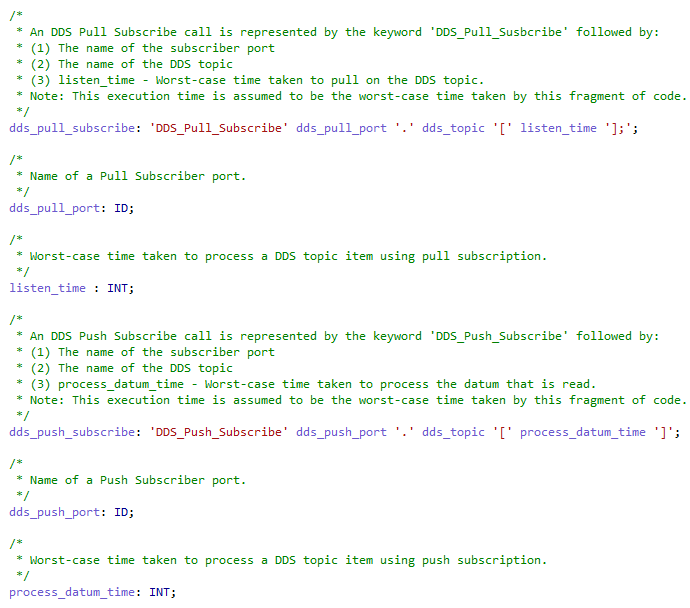
\includegraphics[width=0.99\textwidth]{./figs/Grammar_6}
\caption{DDS Subscribe calls}
\label{fig:grammar6}
\vspace{-0.2in}
\end{figure}
\vspace{0.1in}

\subsection{Control Loops}

\begin{figure}[ht]
\centering
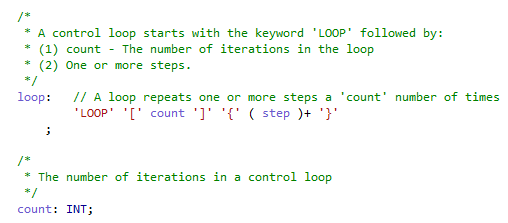
\includegraphics[width=0.70\textwidth]{./figs/Grammar_7}
\caption{Control Loops in the Business Logic}
\label{fig:grammar7}
\vspace{-0.2in}
\end{figure}
\vspace{0.1in}


\section{Modeling the Sensor and Trajectory Planner Operations}

As shown in Figure \ref{fig:tpa}, the user needs to model three component operations - the timer operation on the Sensor, the facet operation on the Sensor and the DDS Push Subscribe operation on the Trajectory Planner. 

\subsection{Sensor Timer Operation}

\begin{figure}[ht]
\centering
\includegraphics[width=0.75\textwidth]{./figs/tpa_timerop}
\caption{Sensor Timer Operation}
\label{fig:tpa_timer}
\vspace{-0.2in}
\end{figure}
\vspace{0.1in}

\subsection{Sensor Facet Operation}

\begin{figure}[ht]
\centering
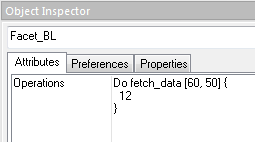
\includegraphics[width=0.60\textwidth]{./figs/TPA_FACETOP}
\caption{Sensor Facet Operation}
\label{fig:tpa_facet}
\vspace{-0.2in}
\end{figure}
\vspace{0.1in}

\subsection{Trajectory Planner DDS Push Subscribe Operation}

\begin{figure}[ht]
\centering
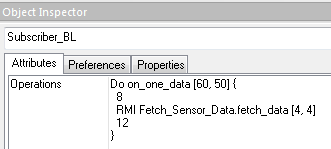
\includegraphics[width=0.70\textwidth]{./figs/TPA_PSH}
\caption{Trajectory Planner DDS Push Subscribe Operation}
\label{fig:tpa_psh}
\vspace{-0.2in}
\end{figure}
\vspace{0.1in}



